
%%%%%%%%%%%%%%%%%%%%%%%%%%%%%%%%%%%%%%%%%%%%%%%%%%%%%%%%
%
% Copyright (c) 2003-2011 by University of Queensland
% Earth Systems Science Computational Center (ESSCC)
% http://www.uq.edu.au/esscc
%
% Primary Business: Queensland, Australia
% Licensed under the Open Software License version 3.0
% http://www.opensource.org/licenses/osl-3.0.php
%
%%%%%%%%%%%%%%%%%%%%%%%%%%%%%%%%%%%%%%%%%%%%%%%%%%%%%%%%

\section{Steady-state Heat Refraction}
\label{STEADY-STATE HEAT REFRACTION}

In this chapter we demonstrate how to handle more complex geometries. 

Steady-state heat refraction will give us an opportunity to investigate some of
the richer features that the \esc package has to offer. One of these is \pycad .
The advantage of using \pycad is that it offers an easy method for developing
and manipulating complex domains. In conjunction with \gmsh we can generate
finite element meshes that conform to our domain's shape providing accurate
modelling of interfaces and boundaries. Another useful function of \pycad is
that we can tag specific areas of our domain with labels as we construct them.
These labels can then be used in \esc to define properties like material
constants and source locations. 

We proceed in this chapter by first looking at a very simple geometry. Whilst a
simple rectangular domain is not very interesting the example is elaborated upon
later by introducing an internal curved interface.

\section{Example 4: Creating the Domain with \pycad}
\label{example4}
\sslist{example04a.py}
We modify the example in Chapter~\ref{CHAP HEAT 2a} in two ways: we look at the
steady state case with slightly modified boundary conditions and use a more
flexible tool to generate the geometry. Let us look at the geometry first. 

We want to define a rectangular domain of width $5 km$ and depth $6 km$ below
the surface of the Earth. The domain is subject to a few conditions. The
temperature is known at the surface and the basement has a known heat flux. Each
side of the domain is insulated and the aim is to calculate the final
temperature distribution.

In \pycad there are a few primary constructors that build upon each other to
define domains and boundaries. The ones we use are:
\begin{python}
from esys.pycad import *
Point() #Create a point in space.
Line() #Creates a line from a number of points.
CurveLoop() #Creates a closed loop from a number of lines.
PlaneSurface() #Creates a surface based on a CurveLoop
\end{python}
So to construct our domain as shown in \reffig{fig:pycad rec}, we first need to
create the corner points. From the corner points we build the four edges of the
rectangle. The four edges then form a closed loop which defines our domain as a
surface. We start by inputting the variables we need to construct the model.
\begin{python}
width=5000.0*m   #width of model
depth=-6000.0*m  #depth of model
\end{python} 

\begin{figure}[ht]
\centerline{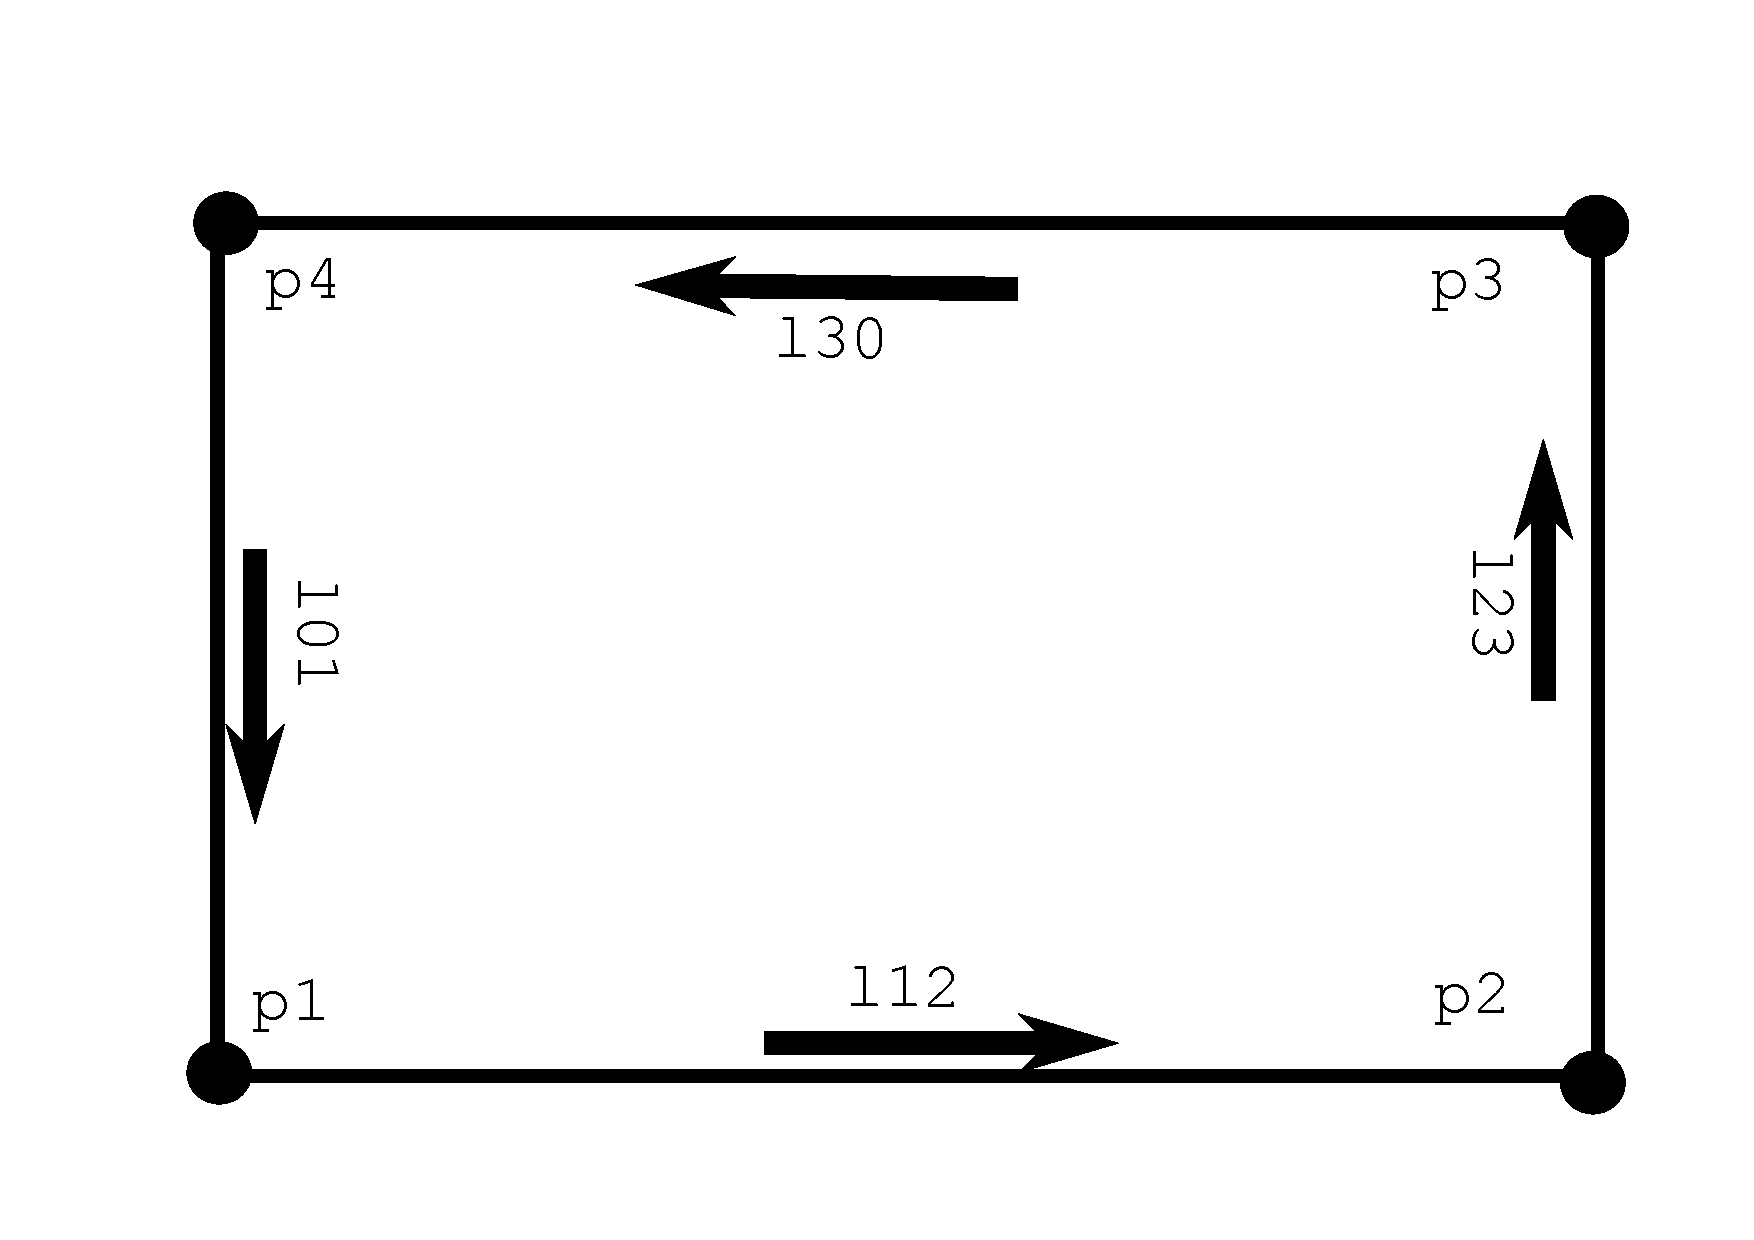
\includegraphics[width=4.in]{figures/pycadrec}}
\caption{Example 4: Rectangular Domain for \pycad}
\label{fig:pycad rec}
\end{figure}

The variables are then used to construct the four corners of our domain, which
from the origin has the dimensions of $5000$ meters width and $-6000$ meters
depth. This is done with the \verb|Point()| function which accepts x, y and z
coordinates. Our domain is in two dimensions so z should always be zero.
\begin{python}
# Overall Domain
p0=Point(0.0,      0.0, 0.0)
p1=Point(0.0,    depth, 0.0)
p2=Point(width, depth, 0.0)
p3=Point(width,   0.0, 0.0)
\end{python}
Now lines are defined using our points. This forms a rectangle around our
domain:
\begin{python}
l01=Line(p0, p1)
l12=Line(p1, p2)
l23=Line(p2, p3)
l30=Line(p3, p0)
\end{python}
Note that lines have a direction. These lines form the basis for our domain
boundary, which is a closed loop.
\begin{python}
c=CurveLoop(l01, l12, l23, l30)
\end{python}
Be careful to define the curved loop in an \textbf{anti-clockwise} manner
otherwise the meshing algorithm may fail.
Finally we can define the domain as
\begin{python}
rec = PlaneSurface(c)
\end{python}
At this point the introduction of the curved loop seems to be unnecessary but
this concept plays an important role if holes are introduced. 

Now we are ready to hand over the domain \verb|rec| to a mesher which
subdivides the domain into triangles (or tetrahedra in 3D). In our case we use
\gmsh. We create an instance of the \verb|Design| class which will handle the
interface to \gmsh: 
\begin{python}
from esys.pycad.gmsh import Design 
d=Design(dim=2, element_size=200*m)
\end{python}
The argument \verb|dim| defines the spatial dimension of the domain\footnote{If
\texttt{dim}=3 the rectangle would be interpreted as a surface in the three
dimensional space.}. The second argument \verb|element_size| defines the element
size which is the maximum length of a triangle edge in the mesh. The element
size needs to be chosen with care in order to avoid very dense meshes. If the
mesh is too dense, the computational time will be long but if the mesh is too
sparse, the modelled result will be poor. In our case with an element size of
$200$m and a domain length of $6000$m we will end up with about $\frac{6000m}{200m}=30$
triangles in each spatial direction. So we end up with about $30 \times 30 =
900$ triangles which is a size that can be handled easily.
The domain \verb|rec| can simply be added to the \verb|Design|;
\begin{python}
d.addItem(rec)
\end{python}
We have the plan to set a heat flux on the bottom of the domain. One can use
the masking technique to do this but \pycad offers a more convenient technique
called tagging. With this technique items in the domain are named using the
\verb|PropertySet| class. We can then later use this name to set values
specifically for those sample points located on the named items. Here we name
the bottom face of the domain where we will set the heat influx:
\begin{python}
ps=PropertySet("linebottom",l12))
d.addItem(ps)
\end{python}
Now we are ready to hand over the \verb|Design| to \FINLEY:
\begin{python}
from esys.finley import MakeDomain
domain=MakeDomain(d)
\end{python}
The \verb|domain| object can now be used in the same way like the return object
of the \verb|Rectangle| object we have used previously to generate a mesh. It
is common practice to separate the mesh generation from the PDE solution.
The main reason for this is that mesh generation can be computationally very
expensive in particular in 3D. So it is more efficient to generate the mesh
once and write it to a file. The mesh can then be read in every time a new
simulation is run. \FINLEY supports this in the following 
way\footnote{An alternative is using the \texttt{dump} and \texttt{load}
functions. They work with a binary format and tend to be much smaller.}:
\begin{python}
# write domain to a text file
domain.write("example04.fly")
\end{python}
and then for reading in another script:
\begin{python}
# read domain from text file
from esys.finley import ReadMesh
domain =ReadMesh("example04.fly")
\end{python}

Before we discuss how to solve the PDE for this problem, it is useful to
present two additional options of the \verb|Design| class. 
These allow the user to access the script which is used by \gmsh to generate
the mesh as well as the generated mesh itself. This is done by setting specific
names for these files: 
\begin{python}
d.setScriptFileName("example04.geo")
d.setMeshFileName("example04.msh")
\end{python}
Conventionally the extension \texttt{geo} is used for the script file of the
\gmsh geometry and the extension \texttt{msh} for the mesh file. Normally these
files are deleted after usage.
Accessing these files can be helpful to debug the generation of more complex
geometries. The geometry and the mesh can be visualised from the command line
using
\begin{verbatim}
gmsh example04.geo  # show geometry
gmsh example04.msh  # show mesh
\end{verbatim}
The mesh is shown in \reffig{fig:pycad rec mesh}.

\begin{figure}[ht]
\centerline{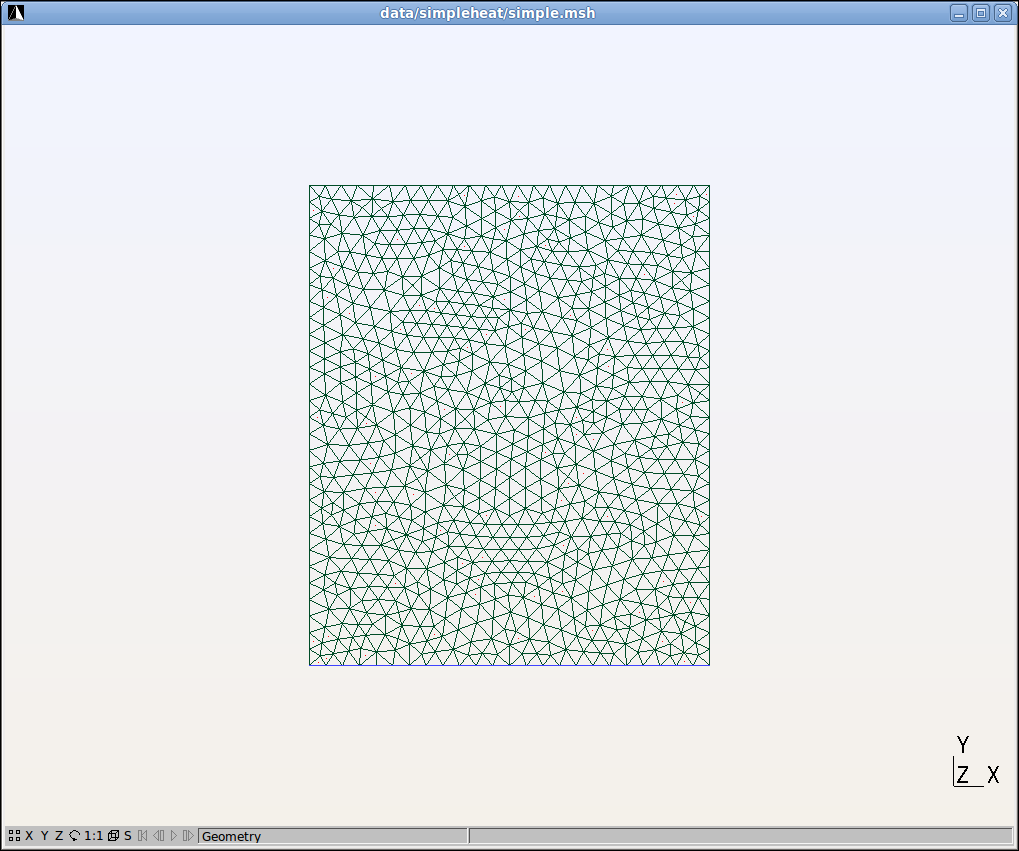
\includegraphics[width=4.in]{figures/simplemesh}}
\caption{Example 4a: Mesh over rectangular domain, see \reffig{fig:pycad rec}}
\label{fig:pycad rec mesh}
\end{figure}
\clearpage

\section{The Steady-state Heat Equation}
\sslist{example04b.py, cblib}
A temperature equilibrium or steady state is reached when the temperature
distribution in the model does not change with time. To calculate the steady
state solution the time derivative term in \refEq{eqn:Tform nabla} needs to be
set to zero;
\begin{equation}\label{eqn:Tform nabla steady}
-\nabla \cdot \kappa \nabla T = q_H
\end{equation}
This PDE is easier to solve than the PDE in \refEq{eqn:hdgenf2}, as no time
steps (iterations) are required. The \verb|D| term from \refEq{eqn:hdgenf2} is
simply dropped in this case.
\begin{python}
mypde=LinearPDE(domain)
mypde.setValue(A=kappa*kronecker(model), Y=qH)
\end{python}
The temperature at the top face of the domain is known as \verb|Ttop|~($=20 C$).
In \refSec{Sec:1DHDv0} we have already discussed how this constraint is added
to the PDE:
\begin{python}
x=Solution(domain).getX()
mypde.setValue(q=whereZero(x[1]-sup(x[1])),r=Ttop)
\end{python}
Notice that we use the \verb|sup| function to calculate the maximum of $y$
coordinates of the relevant sample points.

In all cases so far we have assumed that the domain is insulated which
translates into a zero normal flux $-n \cdot \kappa \nabla T$, see
\refEq{eq:hom flux}. In the modelling set-up of this chapter we want to set
the normal heat flux at the bottom to \verb|qin| while still maintaining
insulation at the left and right face. Mathematically we can express this as
\begin{equation}
-n \cdot \kappa \nabla T = q_{S}
\label{eq:inhom flux}
\end{equation}
where $q_{S}$ is a function of its location on the boundary. Its value
becomes zero for locations on the left or right face of the domain while it has
the value \verb|qin| at the bottom face.
Notice that the value of $q_{S}$ at the top face is not relevant as we
prescribe the temperature here.
We could define $q_{S}$ by using the masking techniques demonstrated
earlier. The tagging mechanism provides an alternative and in many cases more
convenient way of defining piecewise constant functions such as
$q_{S}$. Recall now that the bottom face was denoted with the name
\verb|linebottom| when we defined the domain.
We can use this now to create $q_{S}$;
\begin{python}
qS=Scalar(0,FunctionOnBoundary(domain))
qS.setTaggedValue("linebottom",qin)
\end{python}
In the first line \verb|qS| is defined as a scalar value over the sample points
on the boundary of the domain. It is initialised to zero for all sample points.
In the second statement the values for those sample points which are located on
the line marked by \verb|linebottom| are set to \verb|qin|. 

The Neumann boundary condition assumed by \esc has the form
\begin{equation}\label{NEUMAN 2b}
n\cdot A \cdot\nabla u = y 
\end{equation}
In comparison to the version in \refEq{NEUMAN 2} we have used so far the right
hand side is now the new PDE coefficient $y$. As we have not specified $y$ in
our previous examples, \esc has assumed the value zero for $y$. A comparison of
\refEq{NEUMAN 2b} and \refEq{eq:inhom flux} reveals that one needs to choose
$y=-q_{S}$;
\begin{python}
qS=Scalar(0,FunctionOnBoundary(domain))
qS.setTaggedValue("linebottom",qin)
mypde.setValue(y=-qS)
\end{python}
To plot the results we use the \modmpl library as shown in
\refSec{Sec:2DHD plot}. For convenience the interpolation of the temperature to
a rectangular grid for contour plotting is made available via the
\verb|toRegGrid| function in the \verb|cblib| module. Your result should look
similar to \reffig{fig:steady state heat}.

\begin{figure}[ht]
\centerline{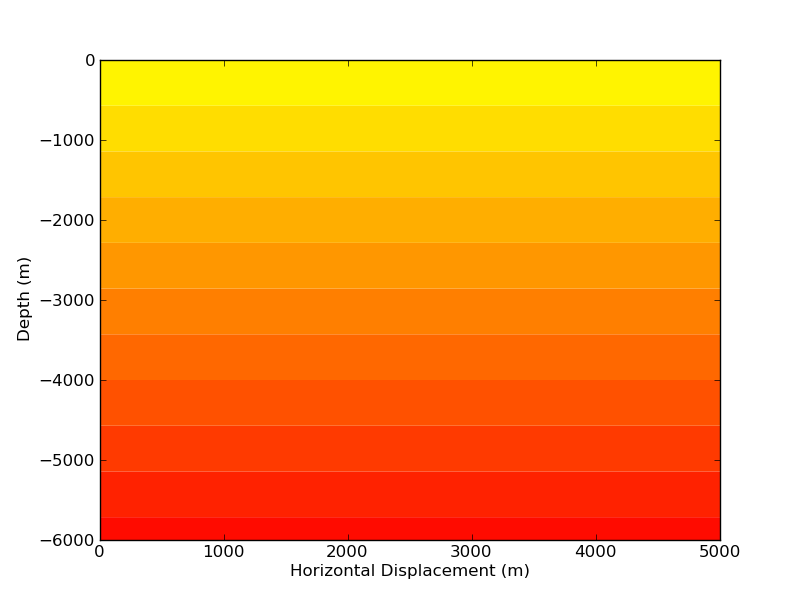
\includegraphics[width=4.in]{figures/simpleheat}}
\caption{Example 4b: Result of simple steady state heat problem}
\label{fig:steady state heat}
\end{figure}
\clearpage

